% CS670 - Reinforcement Learning
% Puddle World Programming Assignment
% Gabriel Dulac-Arnold <gabe@squirrelsoup.net>
% Johannes H. Jensen <johannj@stud.ntnu.no>
\documentclass[a4paper]{article}
%\usepackage{multicol}
\usepackage{graphicx}
\usepackage[top=2cm,nohead,nofoot]{geometry}
\usepackage{subfig}



\graphicspath{{../experiments/graphs/}}

\author{Gabriel Dulac-Arnold $<$gabe@squirrelsoup.net$>$ (CS09F004) \\
Johannes H. Jensen $<$johannj@stud.ntnu.no$>$ (CS09F005)}
\title{CS670 - Reinforcement Learning \\
\emph{Puddle World Programming Assignment}}

\begin{document}
\setlength{\parskip}{2ex}
\maketitle

\section{Q-Learning and Sarsa}

Q-Learning and Sarsa were both trained using a constant exploring probability 
$\epsilon = 0.1$ and learning rate $\alpha = 0.1$ over 10 000 episodes, averaged
over 50 runs.

\subsection{Goal A}

\begin{figure}[htbp!]
\center
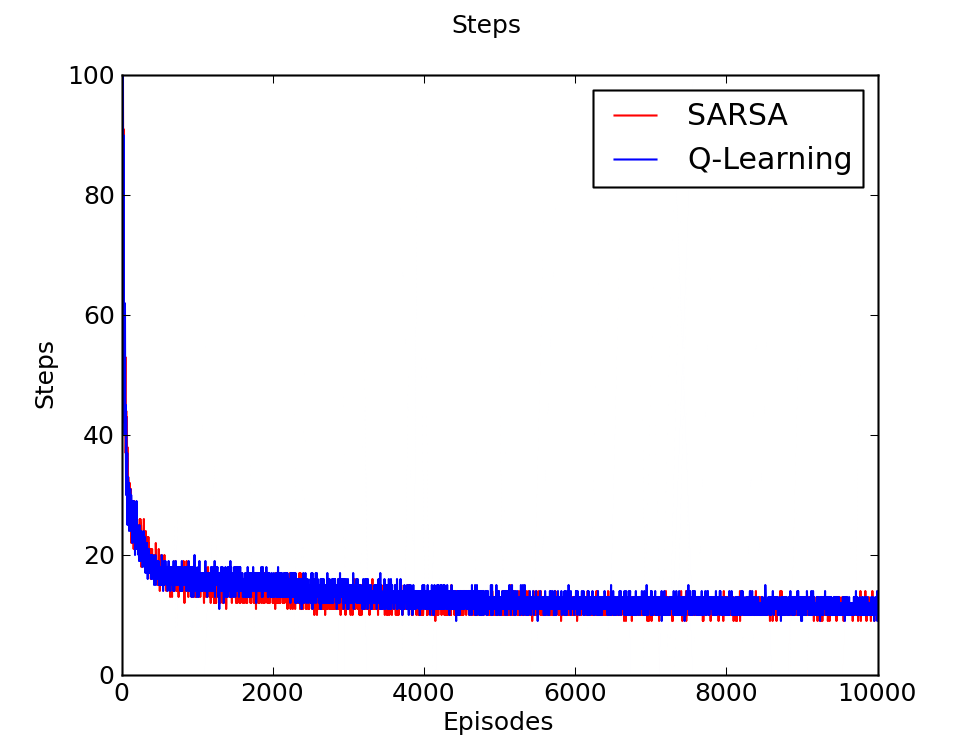
\includegraphics[scale=0.75]{A/steps.png}
\caption{Average number of steps to reach goal}
\end{figure}

\begin{figure}[htbp!]
\center
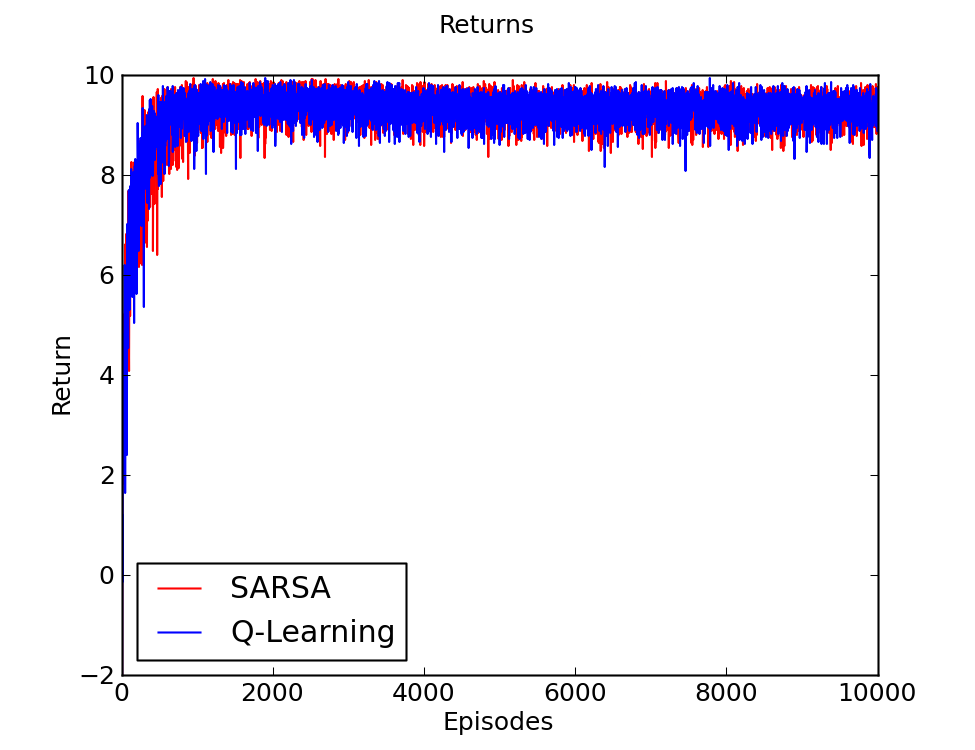
\includegraphics[scale=0.75]{A/returns.png}
\caption{Average reward per episode}
\end{figure}

\begin{figure}[htbp!]
\center
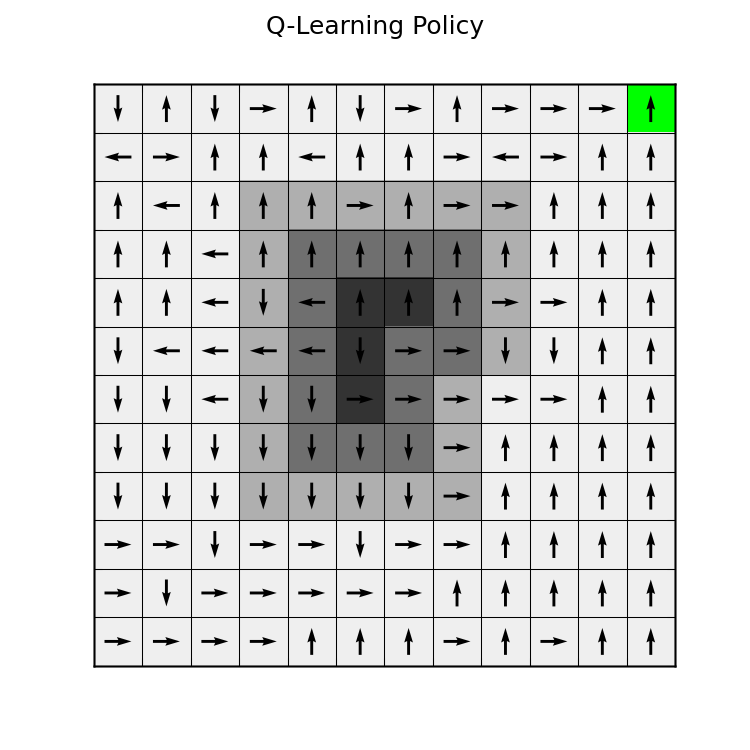
\includegraphics[scale=0.75]{A/Q-Learning-policy.png}
\caption{Policy learned by Q-Learning}
\end{figure}

\begin{figure}[htbp!]
\center
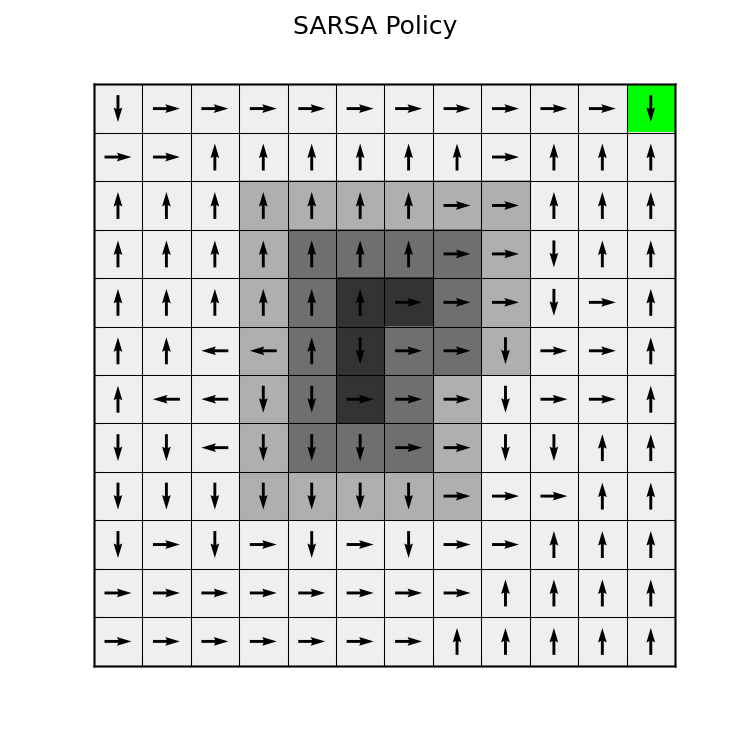
\includegraphics[scale=0.75]{A/SARSA-policy.png}
\caption{Policy learned by Sarsa}
\end{figure}

\newpage
\subsection{Goal B}

\begin{figure}[htbp!]
\center
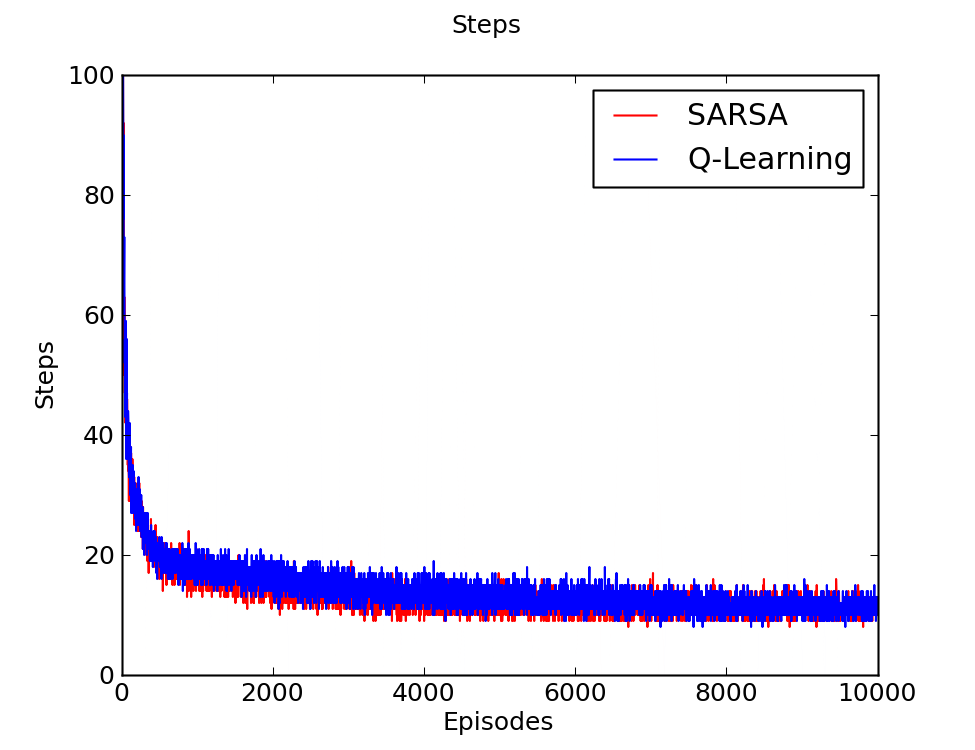
\includegraphics[scale=0.75]{B/steps.png}
\caption{Average number of steps to reach goal}
\end{figure}

\begin{figure}[htbp!]
\center
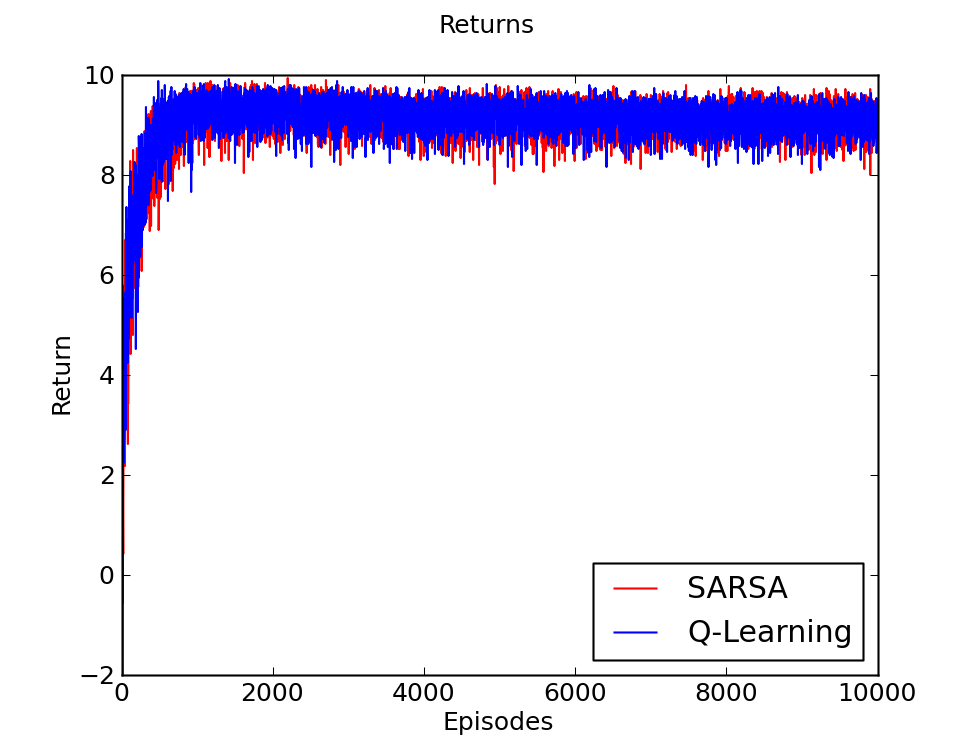
\includegraphics[scale=0.75]{B/returns.png}
\caption{Average reward per episode}
\end{figure}

\begin{figure}[htbp!]
\center
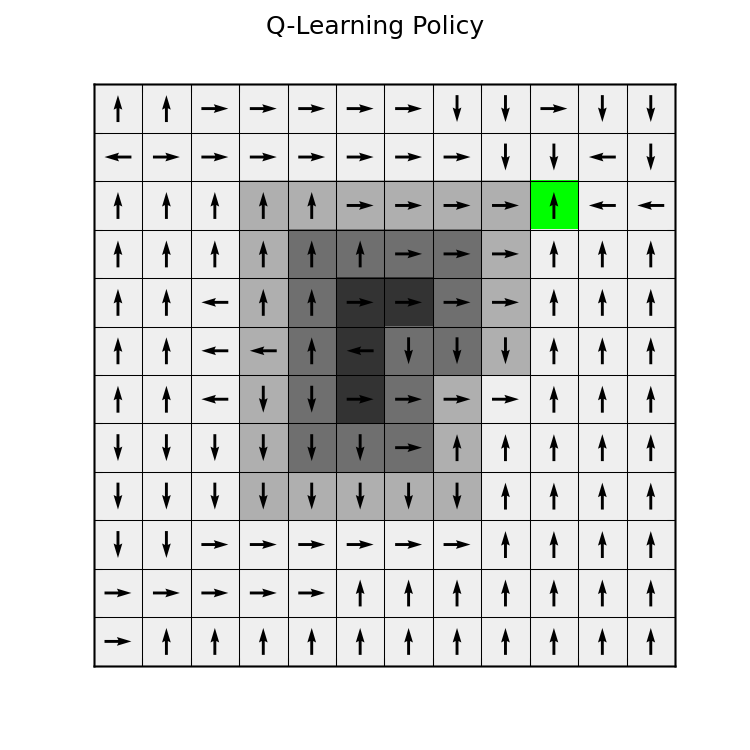
\includegraphics[scale=0.75]{B/Q-Learning-policy.png}
\caption{Policy learned by Q-Learning}
\end{figure}

\begin{figure}[htbp!]
\center
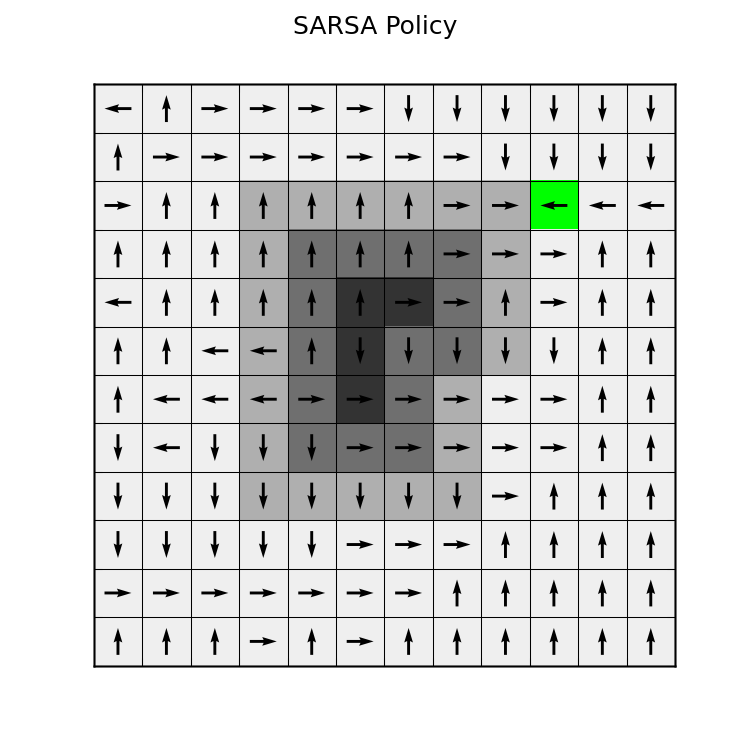
\includegraphics[scale=0.75]{B/SARSA-policy.png}
\caption{Policy learned by Sarsa}
\end{figure}


\newpage
\subsection{Goal C}

\begin{figure}[htbp!]
\center
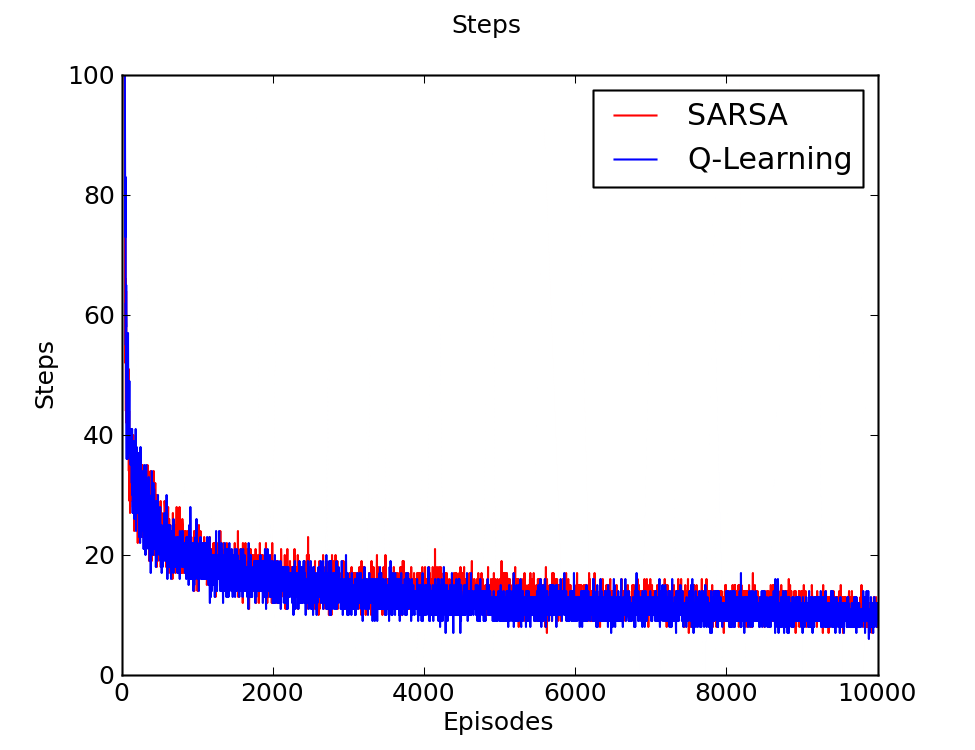
\includegraphics[scale=0.75]{C/steps.png}
\caption{Average number of steps to reach goal}
\end{figure}

\begin{figure}[htbp!]
\center
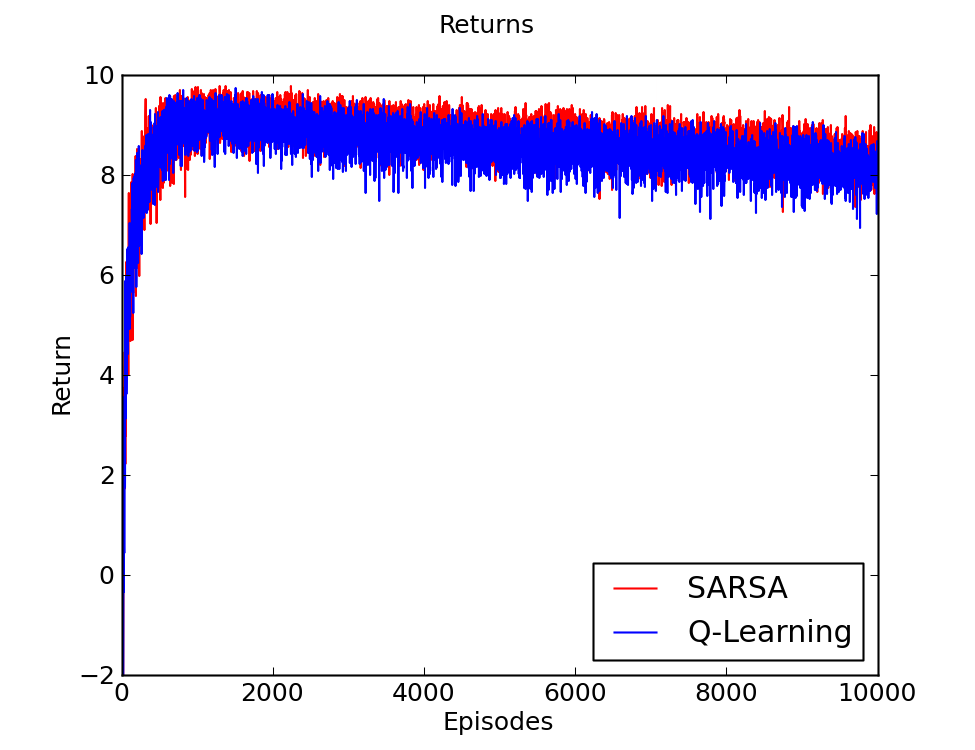
\includegraphics[scale=0.75]{C/returns.png}
\caption{Average reward per episode}
\end{figure}

\begin{figure}[htbp!]
\center
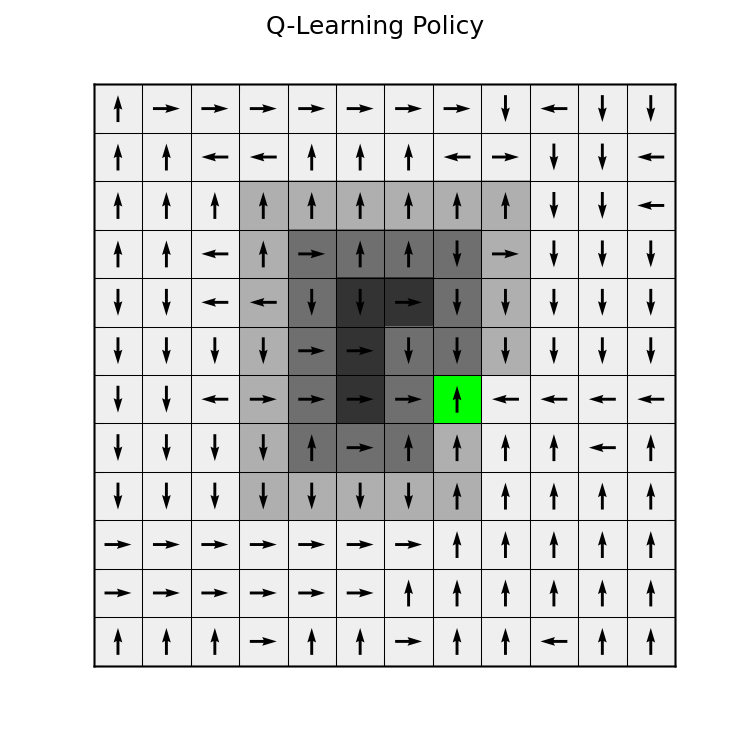
\includegraphics[scale=0.75]{C/Q-Learning-policy.png}
\caption{Policy learned by Q-Learning}
\end{figure}

\begin{figure}[htbp!]
\center
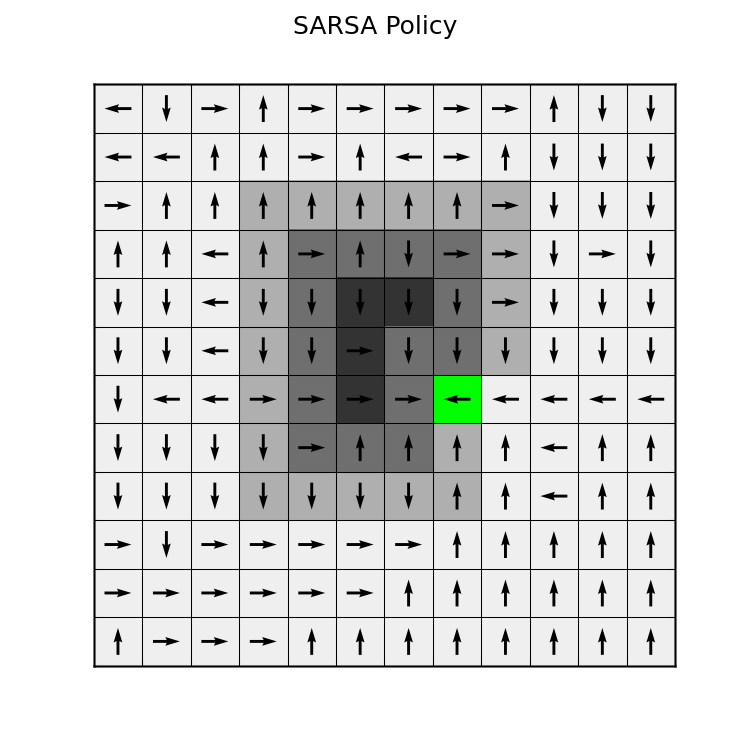
\includegraphics[scale=0.75]{C/SARSA-policy.png}
\caption{Policy learned by Sarsa}
\end{figure}

\newpage

\section{Policy Gradient}

Policy Gradient was run on an environment with deterministic actions using 
learning rate $\alpha = 0.005$ and initial temperature $\tau = 500$ for 5000
episodes, averaged over 30 runs. This method only converged for Goal A.

\begin{figure}[htbp!]
\center
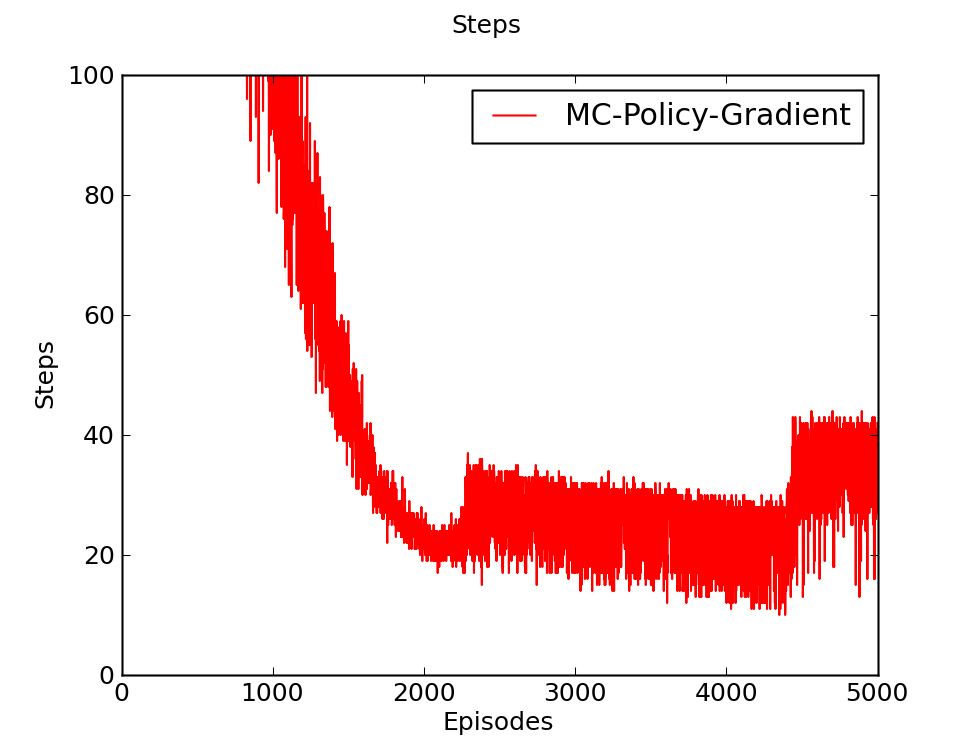
\includegraphics[scale=0.75]{A/pg-steps.png}
\caption{Average number of steps to reach goal}
\end{figure}

\begin{figure}[htbp!]
\center
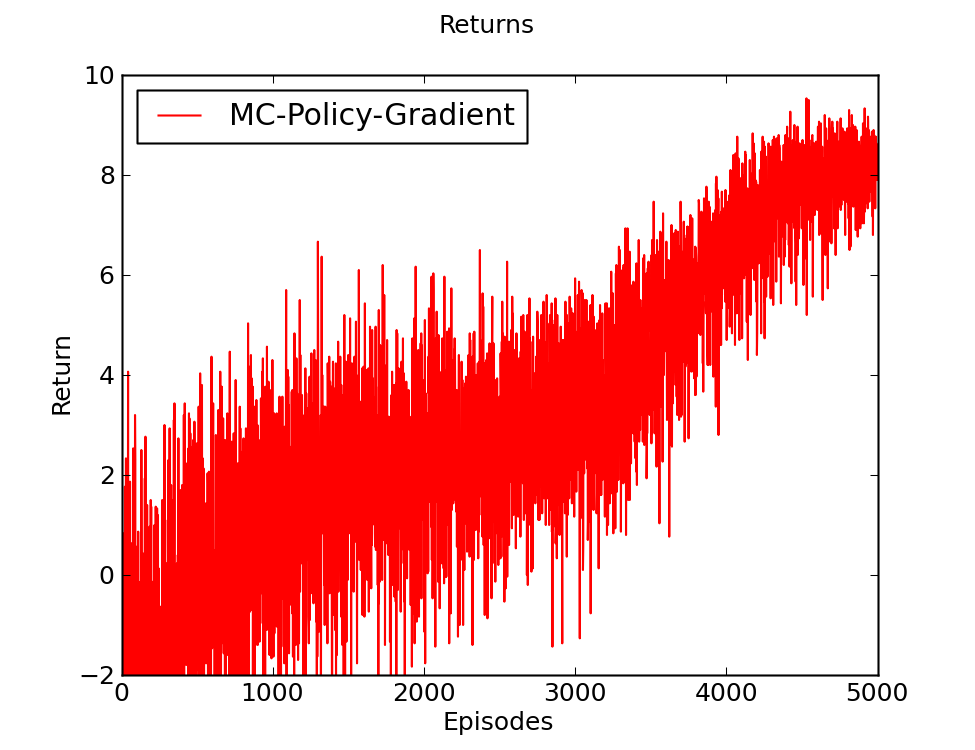
\includegraphics[scale=0.75]{A/pg-returns.png}
\caption{Average reward per episode}
\end{figure}

\begin{figure}[htbp!]
\center
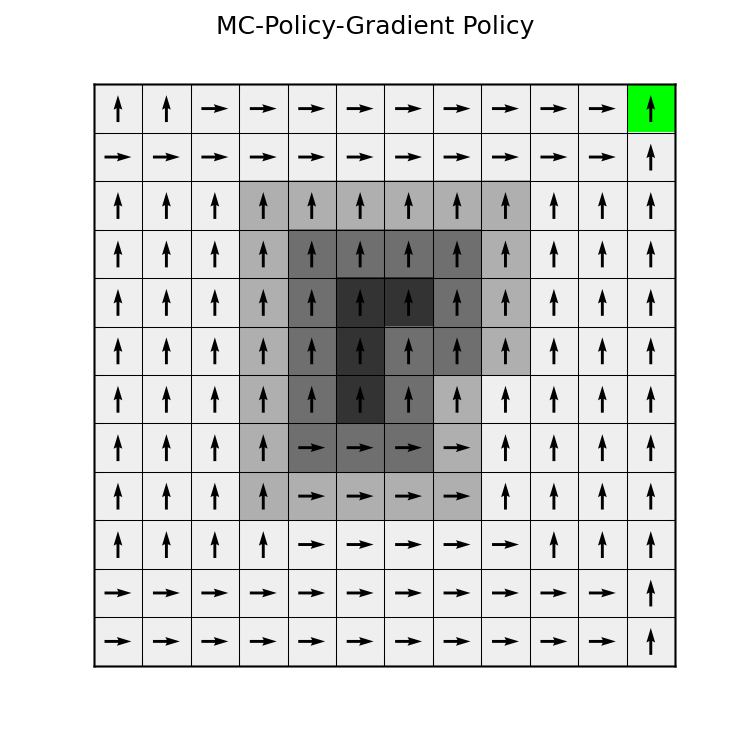
\includegraphics[scale=0.75]{A/MC-Policy-Gradient-policy.png}
\caption{Policy learned by MC Policy Gradient}
\end{figure}


\end{document}
